A measurement of the cross section times branching fration of \ttH (\Hgg)~production is performed by defining regions of the data which are highly enriched in \ttH events. These regions, called ``signal regions'', are constructed through a set of requirements placed on all candidate events. 
The requirements consist of two components: 
(1) a ``loose preselection'', which selects events with at least some of the expected decay products of the \ttH system and 
(2) a selection based on the output of a binary classification algorithm (called ``BDT-bkg''), trained to separate \ttH from the SM background processes. The loose preselection aims to maintain a very high signal efficiency (FIXME: CITE) and provides the phase space in which BDT-bkg is trained.
The BDT-bkg algorithm is trained on MC simulation of signal and background, as well as a data-driven description of some backgrounds. After training the BDT-bkg algorithm, signal regions are constructed by placing requirements on the output of BDT-bkg (on top of the preselection requirements).
Within these signal regions, signal and background models are constructed and a measurement of the \ttH cross section is calculated by performing a simultaneous fit to events in all of the signal regions. 
%Although the loose preselection maintains an efficiency of X\% (FIXME) on \ttH events, the SM background is still far too large to perform a precise measurement of the \ttH cross section. The output of BDT-bkg is then used to construct signal regions.
%
\subsection{The \Hgg Decay Mode}
The analysis targets \ttH events in which the Higgs boson decays into two photons (\Hgg). As the photon is a massless particle, it does not couple directly to the Higgs boson.
Instead, the dominant process through which the Higgs boson decays to two photons involves a top quark loop, as shown in Figure~\ref{fig:hgg_feynman}.
\begin{figure}[h!]
    \centering
    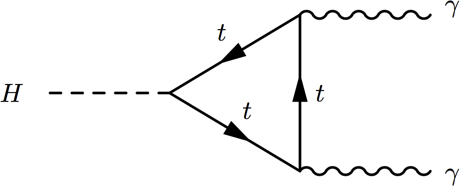
\includegraphics[width=0.6\textwidth]{figures/feynman_diagrams/hgg}
    \caption{To-do}
    \label{fig:hgg_feynman}
\end{figure}
The \Hgg branching ratio is quite small ($\approx 0.2\%$) in comparison to other commonly studied decay modes, but the diphoton channel presents several key advantages.

First, the CMS ECAL provides excellent energy resolution ($\sigma_E/E$) for reconstructed photons, which ranges from 1-5\% \cite{Chatrchyan:2013dga}.
In general, photons with smaller absolute values of pseudorapidity and higher values of the shower shape variable $R_9$ (defined in Section \ref{sec:evt_photon}) are reconstructed with better energy resolution.
The resulting resolution of the invariant mass of diphoton pairs then ranges from 1-2\% for events considered in this analysis.
Exact values for the mass resolution in each signal region are given in Section \ref{sec:sig_bkg_models}.
The mass resolution for other Higgs decay modes is typically much worse.
The CMS observation of the $\text{H} \to \text{b}\bar{\text{b}}$ decay mode, for example, achieved a mass resolution of 10-13\% \cite{Hbb_obs}.
The excellent mass resolution of the diphoton channel contributes to its competitive sensitivity -- the SM background follows a steeply falling distribution as a function of increasing diphoton invariant mass, while \Hgg events are clustered around \mH with a resolution of 1-2\%.
The narrow peak around \mH allows for greater discrimination against the SM background processes.

The second advantage of the diphoton decay channel is the relatively small SM background.
At the LHC, final states with photons or leptons are significantly rarer than final states with hadrons.
Each photon or lepton in a final state introduces another factor of the fine structure constant, $\alpha \approx 1/137$, in the cross section times branching ratio for a given process. 
A crude back of the envelope estimation suggests that final states with $N$ leptons plus photons have characteristic cross sections times branching ratios a factor of $\alpha^{-N}$ times smaller than characteristic cross sections times branching ratios for all-hadronic final states.

Finally, the diphoton decay channel has low systematic uncertainties in comparison to other Higgs decay modes.
Recent \ttH cross section measurements in multilepton and $\text{b}\bar{\text{b}}$ final states reported total systematic uncertainties of FIXME and CITE, while this result reports a systematic uncertainty of FIXME.
The fact that the uncertainty on measurements in the \Hgg channel are dominated by statistical uncertainties casts it as the ``golden channel'' for future Higgs studies in Run 3 of the LHC; the statistical uncertainty on measurements scales roughly with the inverse square root of the luminosity, while the systematic uncertainty remains roughly constant as a function of luminosity.

\subsection{Estimates of Expected Sensitvity} \label{sec:tth_za}
In developing the \ttH analysis, the following question frequently arises: will method A or method B give a better result?
``Method'' may refer to a machine learning algorithm, a description of the SM background, etc.
``Better'' is a subjective matter, but the primary measurement of the \ttH analysis is that of $\mu_{\ttH}$, defined as the ratio of the observed cross section times branching fraction of \ttH (\Hgg) and the predicted cross section times branching fraction:
\begin{equation}
    \mu_{\ttH} = \frac{(\sigma_{\ttH} \times \mathcal B (\Hgg))_{\text{obs}}}{(\sigma_{\ttH} \times \mathcal B (\Hgg))_{\text{SM}}}.
\end{equation}
Therefore, ``better'' is taken to mean ``giving a smaller expected uncertainty on the measurement of $\mu_{\ttH}$''.
The superlative is framed in terms of the expected uncertainty, rather than the observed uncertainty, as the analysis is developed in a blinded fashion to avoid introducing bias.
The full calculation of $\mu_{\ttH}$ involves extensive computing (and human) time, so a simplified measure of the expected uncertainty is used.
For these purposes, we use $Z_A$~\cite{cowan_za}, defined as
\begin{equation}
    Z_A(s,b) = \sqrt{2 \bigg((s+b)\ln(1 + \frac{s}{b})-s\bigg)},
\end{equation}
where $s$ is the number of signal events and $b$ is the number of background events.
In the limit $s<<b$, the Taylor expansion of $Z_A$ gives the familiar $s/\sqrt{b}$:
\begin{equation}
    Z_A(s,b) = \frac{s}{\sqrt{b}}\bigg[1 + \mathcal O \bigg(\frac{s}{b}\bigg) \Bigg].
\end{equation}
The signal yield $s$ is estimated by fitting a Gaussian function to the \mgg distribution of signal MC events and integrating the fitted function over the signal mass window.
The background yield $b$ is estimated by counting the yield of all events in the \mgg sidebands (100 GeV $< \mgg < 120$ GeV, 130 GeV $< \mgg < 180$ GeV) and scaling to the size of the signal mass window.
The signal mass window is taken to be $\mH \pm 1.645 \times \sigma_{\text{eff}}$, with $\sigma_{\text{eff}}$ taken from the fitted Gaussian.
It is not necessary to employ more sophisticated estimates of the signal and background yields (as is done in Sec.~\ref{sec:sig_bkg_models}) because $Z_A$ is only used in comparing the performance of two strategies; the absolute value of $Z_A$ is not relevant.
When quoting an improvement obtained by using a specific method, the value is taken as the percentage difference between the maximum $Z_A$ values obtained by the two methods.
